%% Except where otherwise noted, content in this documentation is Copyright (c)
%% 2015-2019, RTE (http://www.rte-france.com) and licensed under a
%% CC-BY-4.0 (https://creativecommons.org/licenses/by/4.0/)
%% license. All rights reserved.

\documentclass[a4paper, 12pt]{report}

% Latex setup
%%  Copyright (c) 2015-2019, RTE (http://www.rte-france.com)
%%  See AUTHORS.txt
%%  All rights reserved.
%%  This Source Code Form is subject to the terms of the Mozilla Public
%%  License, v. 2.0. If a copy of the MPL was not distributed with this
%%  file, you can obtain one at http://mozilla.org/MPL/2.0/.
%%  SPDX-License-Identifier: MPL-2.0
%%
%%  This file is part of Dynawo, an hybrid C++/Modelica open source time domain
%%  simulation tool for power systems.


%%%%%%%%%%%%%%%%%%%%%%%%%%%%%%%%%%%%%%%%%%%
% Define text and document settings
%%%%%%%%%%%%%%%%%%%%%%%%%%%%%%%%%%%%%%%%%%%

\usepackage{lmodern} % Latin Modern fam­ily of fonts
\usepackage[english]{babel} % English

% Specify encoding
\usepackage[utf8]{inputenc} % Input
\usepackage[T1]{fontenc} % Output

% Document structure setup
\usepackage{titlesec} % To change chapter format
\setcounter{tocdepth}{3} % Add subsubsection in Content
\setcounter{secnumdepth}{3} % Add numbering for subsubsection
\setlength{\parindent}{0pt} % No paragraph indentation

% Avoid numbering starting at each chapter for figures
\usepackage{chngcntr}
\counterwithout{figure}{chapter}

% Change title format for chapter
\titleformat{\chapter}{\Huge\bf}{\thechapter}{20pt}{\Huge\bf}

% To add links on page number in Content and hide red rectangle on links
\usepackage[hidelinks, linktoc=all]{hyperref}
\usepackage[nottoc]{tocbibind} % To add biblio in table of content
\usepackage{textcomp} % For single quote
\usepackage{url} % Allow linebreaks in \url command
\usepackage{listings} % To add code samples

% Define typography
\usepackage{xspace}
\usepackage{dirtree}
\newcommand{\Dynawo}[0]{Dyna$\omega$o\xspace}

% Default listings parameters
\lstset
{
  aboveskip={1\baselineskip}, % A bit of space above
  backgroundcolor=\color{shadecolor}, % Choose the background color
  basicstyle={\ttfamily\footnotesize}, % Use font and smaller size \small \footnotesize
  breakatwhitespace=true, % Sets if automatic breaks should only happen at whitespace
  breaklines=true, % Sets automatic line breaking
  columns=fixed, % Nice spacing -> fixed / flexible
  mathescape=false, % Escape to latex false
  numbers=left, % Where to put the line-numbers
  numberstyle=\tiny\color{gray}, % The style that is used for the line-numbers
  showstringspaces=false, % Do not emphasize spaces in strings
  tabsize=4, % Number of spaces of a TAB
  texcl=false, % Activates or deactivates LaTeX comment lines
  upquote=true % Upright quotes
}

%%%%%%%%%%%%%%%%%%%%%%%%%%%%%%%%%%%%%%%%%%%
% Define plots settings
%%%%%%%%%%%%%%%%%%%%%%%%%%%%%%%%%%%%%%%%%%%

% Macro pack­age for cre­at­ing graph­ics
\usepackage{tikz}
\usepackage{subfigure}
\usepackage{float}

% Draws func­tion plots (based on pgf/tikz)
\usepackage{pgfplots}
\pgfplotsset{enlarge x limits=false, xlabel={\begin{small}$time$ (s)\end{small}}, height=0.6\textwidth, width=1\textwidth}
\pgfplotstableset{col sep=semicolon}

% Define colors
\usepackage{color}
\definecolor{blue}{rgb}{.3,.5,1}
\definecolor{deepblue}{rgb}{0,0,1}
\definecolor{darkblue}{rgb}{0,0,.4}
\definecolor{red}{rgb}{1,0,0}
\definecolor{darkred}{rgb}{.56,0,0}
\definecolor{pink}{rgb}{.933,0,.933}
\definecolor{purple}{rgb}{0.58,0,0.82}
\definecolor{green}{rgb}{0.133,0.545,0.133}
\definecolor{darkgreen}{rgb}{0,.4,0}
\definecolor{gray}{rgb}{.3,.3,.3}
\definecolor{darkgray}{rgb}{.2,.2,.2}
\definecolor{shadecolor}{gray}{0.925}

%%%%%%%%%%%%%%%%%%%%%%%%%%%%%%%%%%%%%%%%%%%
% Define blocks for simple network drawings
%%%%%%%%%%%%%%%%%%%%%%%%%%%%%%%%%%%%%%%%%%%

% Define blocks for newtorks drawings
\usepackage{amsmath} % Add math­e­mat­i­cal fea­tures
\usepackage{schemabloc} % Add block diagram library (french one)

%% Define infinite bus
\tikzset{infinite bus/.pic={
  code={
  \draw (0,0) circle (2) node[inner sep=0, outer sep=0] {{$\infty$}};
  \draw (2,0) --++ (2,0);
  }
  }
}

%% Define transformer
\tikzset{transfo/.pic={
  code={
  \draw (0,0) circle (2);
  \draw (2,0) circle (2);
  \draw (4,0) --++ (4,0);
  \draw (-2,0) --++ (-4,0);
  }
  }
}

%% Define generator
\tikzset{generator/.pic={
  code={
    \draw (0,0) circle (2);
    \draw (0,0) arc (0:180:0.5);
    \draw (0,0) arc (180:360:0.5);
    \draw (-2,0) --++ (-2,0);
  }
  }
}

%% Define generator controls
\tikzset{VR/.pic={
  code={
  \draw (0,0) circle (2) node[inner sep=0, outer sep=0] {{VR}};
  }
  }
}

%% Define SVarC
\tikzset{SVarC/.pic={
  code={
  \draw (0,0) circle (4) node[inner sep=0, outer sep=0] {{SVarC}};
  }
  }
}


\begin{document}

\title{\Dynawo Introduction Documentation}
\date\today

\maketitle
\tableofcontents

\chapter{Introduction}

\section{What is \Dynawo ?}

\textbf{\Dynawo is an hybrid C++/Modelica open source suite of simulation tools for power systems. It aims at providing power system stakeholders with a transparent, flexible, interoperable and robust suite of simulation tools that could ease collaboration and cooperation in the power system community.} \\

To achieve this goal, \textbf{\Dynawo is based on two mains principles}: the use of a high-level modelling language \href{https://modelica.org/} {\underline{Modelica}} and a strict separation between the modelling and the solving parts. \\

It is an ongoing project based on previous works conducted particularly in two R\&D European projects: \href{http://www.fp7-pegase.com/}{\underline{Pegase}} and \href{http://www.itesla-project.eu/}{\underline{iTesla}}. These projects have contributed to the choices that are the basis upon which \Dynawo is built: they proved the usability of the Modelica language for power system simulations and contributed to the development of numerical resolution strategies that are integrated into \Dynawo. \\

\begin{figure}[h!]
\centering
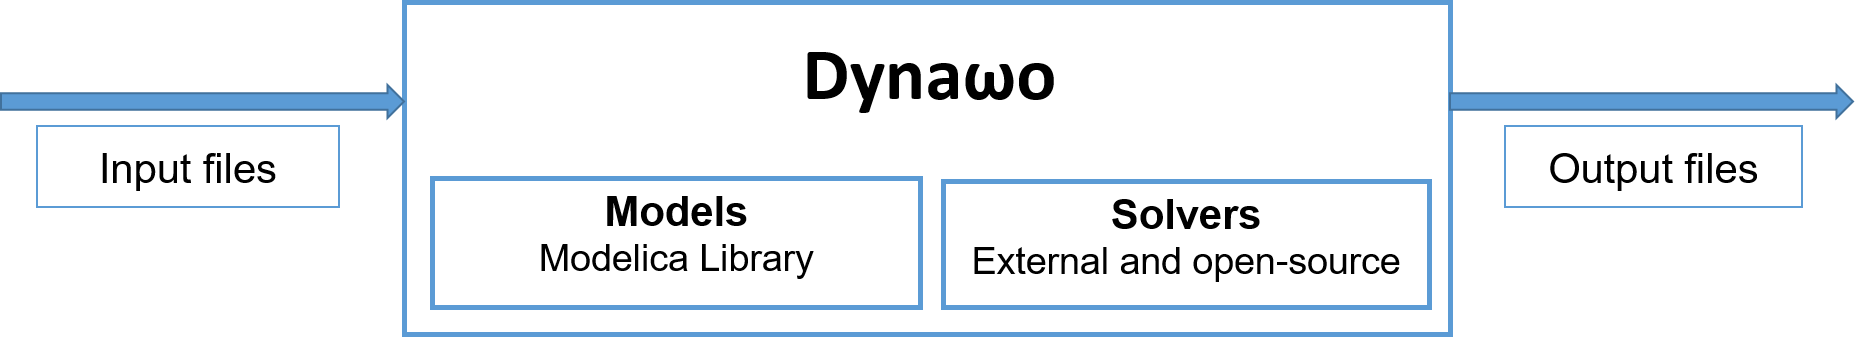
\includegraphics[width=\textwidth]{../resources/DynawoModelSolverLight.png}
\caption{Separation between modelling and solving parts in \Dynawo}
\end{figure}


\textbf{\Dynawo 's primary focus has been on long-term and short-term stability studies} but the very encouraging results obtained and the flexibility of the approach led to \textbf{an extension of the initiative. \Dynawo is now evolving towards a complete and coherent suite of simulation tools}, sharing the same philosophy:
\begin{itemize}
\item DynaFlow for steady-state calculations
\item DySym for short-circuit calculations
\item DynaWaltz for long-term stability simulations
\item DynaSwing for short-term stability studies
\item DynaWave for stability studies and system design with a high-penetration of power-electronics based components (quasi-EMT)
\end{itemize}

\begin{figure}[h!]

\includegraphics[width=\textwidth]{../resources/DynawoLogos.png}
\end{figure}

\begin{figure}[h!]
\centering
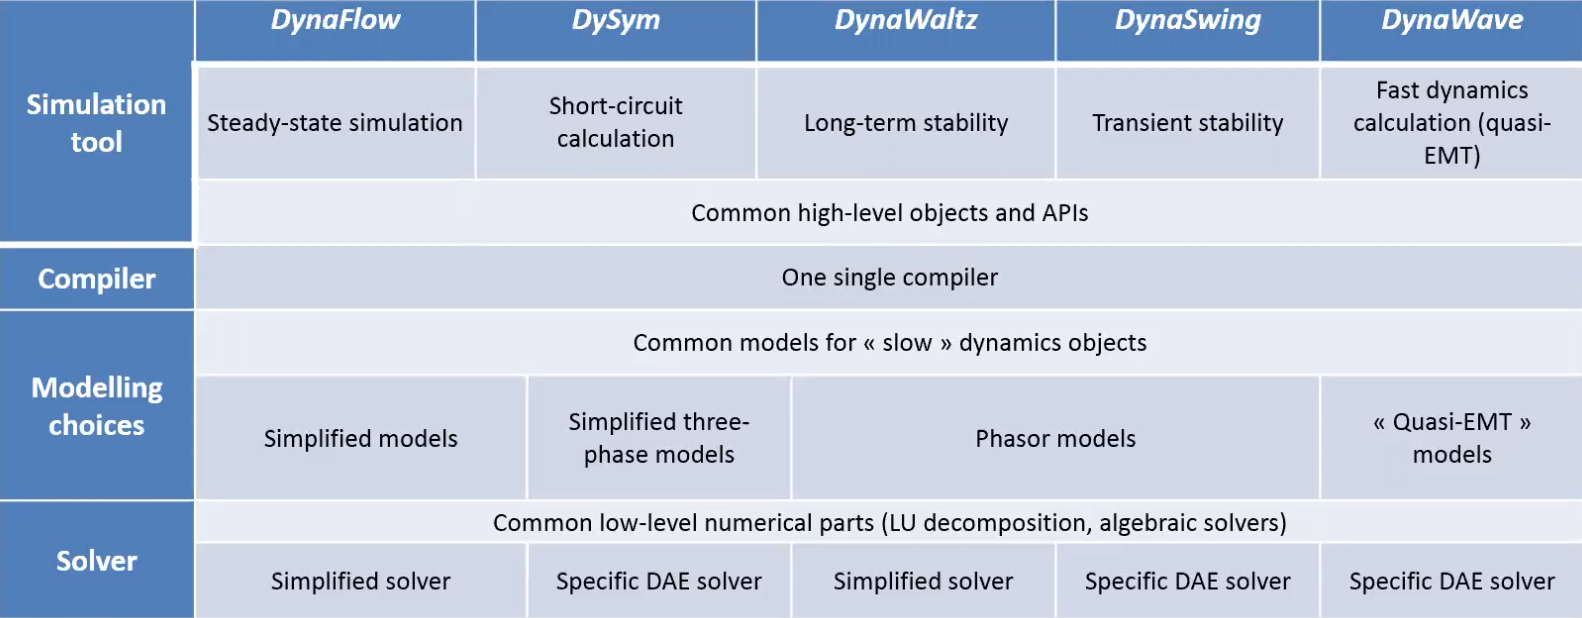
\includegraphics[width=\textwidth]{../resources/DynawoInitiative.png}
\caption{High-level vision of the \Dynawo initiative}
\end{figure}

\textbf{Only validated models, numerical methods and test cases are included into this release.} We plan to release additional features in the near future, including for example additional models (standard wind and solar power plant models, new regulations for synchronous machines, etc.), or new test cases (Nordic32 test case, large-scale test cases).

In addition to the \Dynawo repository, you can have a look to our new dynawo-algorithms repository - \url{https://github.com/dynawo/dynawo-algorithms} -, enabling to launch contingency analysis, voltage margin  or critical clearing time calculations. \\

\Dynawo is licensed under the terms of the \href{http://mozilla.org/MPL/2.0}{\underline{Mozilla Public License, v2.0}}.
The source code is hosted into a \href{https://github.com/dynawo/dynawo} {\underline{GitHub repository}}. \\

\section{Getting started}

To get started with \Dynawo , different possibilities exist, depending on your background and what you want to do:
\begin{itemize}
\item If you are interested in the models available and want to have a look to them, please open the \Dynawo Modelica library into OpenModelica and run the full Modelica examples provided with the library.
\item If you want to launch simulations and examples with \Dynawo and observe the performances, you can use the pre-built distribution and run the simulations provided into the examples directory.
\item If you want to modify the tool yourself or try new methods and models, please checkout the repository and build it.
\end{itemize}

\section{Changes from previous versions}

\subsection{Changes from v1.3.0}

\underline{Main changes:}
\begin{itemize}
\item Additional standard models (IEEE regulations, WECC RES) and simplified models (SVarC, HVDC, etc.)
\item Addition of a trapezoidal solver and refactoring of the solvers architecture
\item API update with two new APIs: final state values and lost equipments.
\item Improved support of the Modelica language
\item Drop of C++98 and MacOS support
\end{itemize}

\underline{New features:}
\begin{itemize}
\item Fault on a bus without injection
\item New APIs for lost equipments and final state values
\end{itemize}

\underline{New models:}
\begin{itemize}
\item Additional IEEE standard regulations
\item WECC Wind Turbine and Photovoltaics models
\item Steady-state/simplified models for HVDC and SVarC components
\end{itemize}

\underline{Solvers:}
\begin{itemize}
\item New fixed-time step solver using the trapezoidal method
\item Refactoring of the solvers code
\end{itemize}

\underline{3rd Party:}
\begin{itemize}
\item Sundials update to version 5.3.0
\item Adept update to version 2.0.8
\item Improved support of the Modelica language
\end{itemize}

\underline{Test cases:}
\begin{itemize}
\item ENTSO-E digital controller test case in full Modelica and \Dynawo
\item WSCC 9 bus test case into \Dynawo
\item WECC RES test cases in full Modelica and \Dynawo
\end{itemize}


\subsection{Changes from v1.2.2}

\underline{Main changes:}
\begin{itemize}
\item Use of powsybl-iidm4cpp 1.4.0 and boost 1.70
\item New TapChangerBlocking model to monitor up to five voltage levels
\item Correct modeling of batteries
\item Add a script to automatically filter output timelines to ease readability
\item Add the possibility to consider multiple voltage levels in power criteria
\end{itemize}

\subsection{Changes from v1.2.1}

\underline{Main changes:}
\begin{itemize}
\item Improvement of solvers: minimization of residuals and discrete variable evaluations
\item Check criteria at the end of a simulation
\item Possibility to run multiple simulations in multi-threading (thread-safety)
\item Reduction of memory footprint
\end{itemize}

\subsection{Changes from v1.2.0}

\underline{Main changes:}
\begin{itemize}
\item Creation of an example directory with additional test cases
\item Steady-state calculation models release (restorative load, generators, frequency regulation model - Signal N-, HVDCPTanPhi and HVDCPV)
\item Performance improvement up to 20 \% on large-scale simulations (variables simplification, algorithm optimization and implementation improvements)
\item Modeling robustness (handling bad topology, propagation of disconnection signals, data handling improvement)
\end{itemize}

\underline{New features:}
\begin{itemize}
\item New criteria system
\item Complete log refactoring
\end{itemize}

\underline{New models:}
\begin{itemize}
\item HVDC Standard model
\item Shackshaft saturation model
\item Steady-state models
\end{itemize}

\underline{3rd Party:}
\begin{itemize}
\item Improvement in Adept integration (better complex handling and support of CombiTable)
\item Python scripts adaptation to Python 3
\item Modelica utilities integration
\end{itemize}

\underline{Test cases:}
\begin{itemize}
\item Full OM grid forming converter and HVDC test cases (in the examples package of the Dynawo library)
\item Examples section in Dynawo (Steady-state calculation examples - DynaFlow, long-term stability examples - DynaWaltz, transient stability examples - DynaSwing).
\end{itemize}

\subsection{Changes from v1.1.0}

\underline{New features:}
\begin{itemize}
\item Windows and MacOS portability (compilation with Visual Studio 2019)
\item Numerical robustness on severe events (automatic mode generation from Modelica models)
\item Performances improvement (generation of aliased and calculated variables from Modelica)
\end{itemize}

\underline{New models:}
\begin{itemize}
\item Source models (injector BG, injector Id/Iq, converter)
\item Network models (ideal switch, bus and dynamic line)
\item Control models (Grid forming controls, PLL)
\end{itemize}

\underline{3rd parties:}
\begin{itemize}
\item End of compatibility with OpenModelica 1.9.4
\item Integration of Modelica 3.2.3
\end{itemize}

\underline{Additional test cases:}
\begin{itemize}
\item IEEE14 Fault test case
\end{itemize}

\end{document}
